\setkeys{Gin}{keepaspectratio}

\newcommand{\smathm}[1]{\scalebox{0.35}{$#1$}}

\begin{figure*}[t]
\centering

\begin{adjustbox}{max width=\textwidth}
\begin{tikzpicture}[
    x=1cm,
    y=1cm,
    stage/.style={
    draw=gray!65,
    dashed,
    rounded corners=4pt,
    fill=gray!5,
    line width=0.3pt,
    inner sep=0pt
},
branch/.style={
    draw=gray!55,
    rounded corners=3pt,
    fill=white,
    line width=0.3pt,
    inner sep=0pt
},
branchtitle/.style={
    font=\fontsize{3.5}{4}\selectfont,
    anchor=west,
    inner sep=0pt
},
prompt/.style={
    draw=gray!45,
    rounded corners=2pt,
    fill=white,
    line width=0.3pt,
    align=left,
    inner sep=2pt
},
img/.style={
    inner sep=0pt,
    outer sep=0pt,
    anchor=center
},
forward/.style={
    -{Stealth[length=1.4mm]},
    line width=0.4pt
},
connector/.style={
    line width=0.4pt
},
modelbox/.style={
    draw=gray!60,
    rounded corners=4pt,
    fill=gray!25,
    line width=0.4pt,
    inner sep=0pt
},
trainmodule/.style={
    draw=black,
    fill=red!15,
    line width=0.4pt,
    align=center,
    font=\tiny,
},
ie/.style={
    trainmodule,
    trapezium,
    trapezium left angle=75,
    trapezium right angle=75,
    shape border rotate=270,
    minimum width=0.3cm,
    minimum height=0.4cm,
    inner sep=0pt
},
mlp/.style={
    trainmodule,
    rectangle,
    minimum width=0.2cm,
    minimum height=0.305cm,
    inner sep=0pt
},
llm/.style={
    trainmodule,
    rectangle,
    minimum width=0.5cm,
    minimum height=0.6cm,
    inner sep=0pt
}
]

\node[
    stage,
    anchor=south west,
    minimum width=3.62cm,
    minimum height=2.75cm
] (sftstage) at (0,0) {};

\node[
    font=\bfseries\tiny,
    anchor=south west,
    inner sep=0pt
] at ($(sftstage.north west)+(0,-0.00cm)+(0,0.04cm)$)
{1) Multi-task SFT};

\node[
    branch,
    anchor=north west,
    minimum width=1.7cm,
    minimum height=1.21cm
] (reconstructionbranch)
at ($(sftstage.north west)+(0.10cm,-0.10cm)$) {};

\node[
    img,
    anchor=north
] (reconstructionimage)
at ($(reconstructionbranch.north)+(0,-0.10cm)$)
{%
    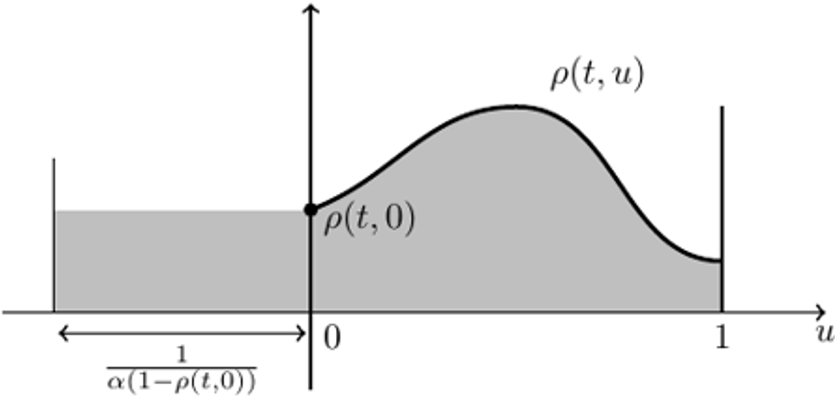
\includegraphics[
        width=1.4cm,
        height=1.4cm
    ]{structure/method_figures/source_target_recon_sft_2.png}%
};

\node[
    branchtitle,
    anchor=north west
] (reconstructiontitle)
at ($(reconstructionbranch.north west)+(0.05cm,-0.04cm)$)
{DaTikZ-V4};

\node[
    prompt,
    anchor=north,
    text width=1.45cm,
    minimum height=0.35cm,
    font=\fontsize{3.2}{3.7}\selectfont
] (reconstructionprompt)
at ($(reconstructionimage.south)+(0,-0.02cm)$)
{%
    This is an image of a scientific figure.
    Reconstruct it in TikZ.
};

\node[
    branch,
    anchor=north west,
    minimum width=2.95cm,
    minimum height=1.23cm
] (editingbranch)
at ($(reconstructionbranch.south west)+(0,-0.10cm)$) {};

\node[
    img,
    anchor=north
] (editingimage)
at ($(editingbranch.north)+(0,-0.05cm)$)
{%
    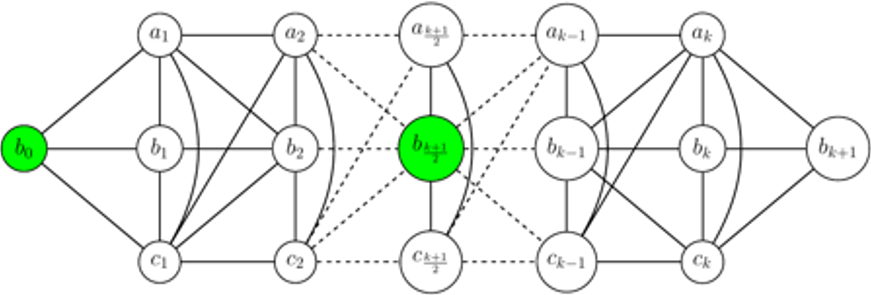
\includegraphics[
        width=1.8cm,
        height=1.8cm
    ]{structure/method_figures/source_edit_sft.png}%
};

\node[
    branchtitle,
    anchor=north west
] (editingtitle)
at ($(editingbranch.north west)+(0.05cm,-0.04cm)$)
{DaEdiTikZ};

\node[
    prompt,
    anchor=north,
    text width=2.70cm,
    minimum height=0.50cm,
    font=\fontsize{3.2}{3.7}\selectfont
] (editingprompt)
at ($(editingimage.south)+(0,-0.02cm)$)
{%
    This is an image of a scientific figure.
    Reconstruct it in TikZ and apply the following changes:
    Remove the entire bottom row of nodes and all edges
    connected to them...
};

\node[
    modelbox,
    anchor=west,
    minimum height=1.0cm,
    minimum width=1.5cm,
] (vlmbox)
at ($(reconstructionbranch.east)+(0.2cm,0.0cm)$) {};

\node[
    branchtitle,
    anchor=south west
] (vlmtitle)
at ($(vlmbox.south west)+(0.05cm,0.04cm)$)
{VLM};

\node[
    ie,
    anchor=north west
] (imageencoder)
at ($(vlmbox.north west)+(0.09cm,-0.17cm)$)
{IE};

\node[
    circle,
    fill=black,
    inner sep=0.7pt
] (Portal)
at ($(imageencoder.south)+(0,-0.2cm)$) {};

\draw[
    connector,
    densely dotted
]
(imageencoder.south) -- (Portal.north);

\node[
    mlp,
    anchor=north west
] (mlpconnector)
at ($(imageencoder.north east)+(0.14cm,0)$)
{C};

\node[
    llm,
    anchor=north west
] (llmdecoder)
at ($(mlpconnector.north east)+(0.10cm,0)$)
{LM};

\draw[connector]
    (imageencoder.east)
    --
    (mlpconnector.west);

\draw[connector]
    (mlpconnector.east)
    --
    (llmdecoder.west |- mlpconnector.east);

\draw[forward]
    (editingbranch.east)
    -|
    ($(vlmbox.south)+(0.45cm,0)$);

\draw[forward]
    (reconstructionbranch.east)
    --
    (vlmbox.west);

\tikzset{
    rlvlm/.style={
        draw=black,
        fill=red!15,
        rounded corners=3pt,
        line width=0.4pt,
        minimum width=0.78cm,
        minimum height=0.58cm,
        align=center,
        font=\tiny
    },
    judgevlm/.style={
        draw=black,
        fill=blue!15,
        rounded corners=3pt,
        line width=0.4pt,
        minimum width=1.0cm,
        minimum height=0.744cm,
        align=center,
        font=\scriptsize
    },
    compilerbox/.style={
        draw=gray!60,
        fill=gray!10,
        rounded corners=3pt,
        line width=0.4pt,
        inner sep=2pt,
        minimum width=1.78cm,
        minimum height=1.65cm,
        align=left
    },
    rolloutbox/.style={
        draw=gray!55,
        fill=white,
        rounded corners=3pt,
        line width=0.3pt,
        inner sep=0pt,
        minimum width=2.90cm,
        minimum height=0.83cm
    },
    frozenie/.style={
        ie,
        fill=blue!15
    }
}

\node[
    stage,
    anchor=north west,
    minimum width=10.2cm,
    minimum height=2.75cm
] (rlstage)
at ($(sftstage.north east)+(0.12cm,0)$) {};

\node[
    font=\bfseries\tiny,
    anchor=south west,
    inner sep=0pt
] (rltitle)
at ($(rlstage.north west)+(0,0.04cm)$)
{2) Multi-Reward RL with GDPO};

\node[
    branch,
    anchor=north west,
    minimum width=1.80cm,
    minimum height=2.55cm
] (rlinput)
at ($(rlstage.north west)+(0.10cm,-0.10cm)$) {};

\node[
    img,
    anchor=north
] (rlsource)
at ($(rlinput.north)+(0,-0.05cm)$)
{%
    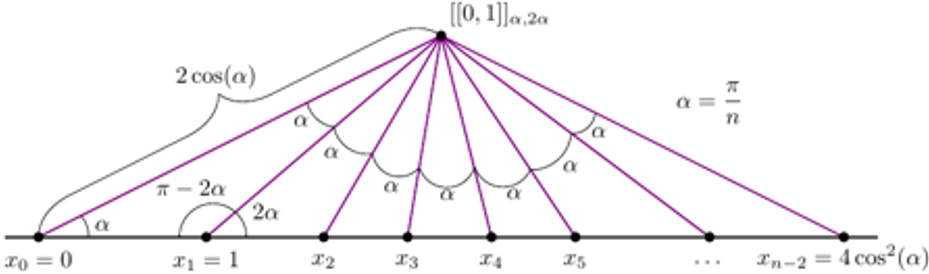
\includegraphics[
        width=1.71cm,
        height=1.20cm
    ]{structure/method_figures/source_rl_new.png}%
};

\node[
    prompt,
    anchor=north,
    text width=1.52cm,
    minimum height=0.85cm,
    font=\fontsize{2.5}{3}\selectfont
] (rlprompt)
at ($(rlsource.south)+(0,-0.03cm)$)
{%
...The label at the top vertex (Mid) is changed from \smathm{[[0,1]]_{\alpha,2\alpha}} to \smathm{[[0,1]]_{\alpha(i+1),\alpha(j+1)}}.
The label for the first point on the left (\smathm{x_0}) is changed from \smathm{x_0 = 0} to \smathm{x_0}.
The label for the second point (\smathm{x_1}) is changed from \smathm{x_1 = 1} to \smathm{x_1}.
The label for the third point (\smathm{x_2}) is changed from \smathm{x_2} to \smathm{\dots}.
The label for the fourth point (\smathm{x_3}) is changed from \smathm{x_3} to \smathm{x_i = 0}.
The label for the fifth point (\smathm{x_4}) is changed from \smathm{x_4} to \smathm{\dots}.
The label for the sixth point (\smathm{x_5}) is changed from \smathm{x_5} to \smathm{x_j = 1}.
The label for the last point on the right (\smathm{x_{n-2}}) is changed from \smathm{x_{n-2} = 4\cos^2(\alpha)} to \smathm{x_{n-2}}.
The brace annotation on the left side indicating the length \smathm{2\cos(\alpha)} is removed...
};

\node[
    star,
    fill=black,
    inner sep=0.7pt
] (RLPortalStar)
at ($(rlinput.east)+(0.2,0.7cm)$) {};

\draw[
    connector,
    densely dotted
]
($(rlinput.east)+(0.0,0.7cm)$) -- (RLPortalStar.west);

\node[
    rlvlm,
    anchor=west
] (rlvlm)
at ($(rlinput.east)+(0.20cm,0)$)
{VLM};

\draw[forward]
    (rlinput.east)
    --
    (rlvlm.west);

\node[
    compilerbox,
    anchor=west
] (compiler)
at ($(rlvlm.east)+(0.20cm,0)$)
{%
    \begin{minipage}{2.01cm}
        \centering

        {\fontsize{4.3}{4.8}\selectfont
        \LaTeX\ Rendering Engine
        }

        \vspace{-9pt}
        \rule{\linewidth}{0.25pt}
        \vspace{-21pt}

        \begin{tikzpicture}[baseline]
            \node[
                anchor=north west,
                inner sep=0pt
            ] (backcode) at (0.06cm,-0.06cm) {%
                \begin{tcolorbox}[
                    enhanced,
                    colback=orange!10,
                    colframe=orange!45,
                    boxrule=0.3pt,
                    arc=2pt,
                    left=0pt,
                    right=0pt,
                    top=0pt,
                    bottom=0pt,
                    boxsep=0pt,
                    width=1.96cm
                ]
                    \lstinputlisting[
                        language=,
                        breaklines=true,
                        breakautoindent=false,
                        breakindent=0pt,
                        columns=fullflexible,
                        keepspaces=true,
                        tabsize=1,
                        showstringspaces=false,
                        aboveskip=0pt,
                        belowskip=0pt,
                        xleftmargin=0pt,
                        basewidth=0.34em,
                        basicstyle=\fontsize{1.3}{1.5}\selectfont\ttfamily
                    ]{structure/method_figures/predicted_tikz.tex}
                \end{tcolorbox}
            };

            \node[
                anchor=north west,
                inner sep=0pt
            ] (frontcode) at (0,0) {%
                \begin{tcolorbox}[
                    enhanced,
                    colback=green!5,
                    colframe=green!50,
                    boxrule=0.3pt,
                    arc=2pt,
                    left=0pt,
                    right=0pt,
                    top=0pt,
                    bottom=0pt,
                    boxsep=0pt,
                    width=1.96cm
                ]
                    \lstinputlisting[
                        language=,
                        breaklines=true,
                        breakautoindent=false,
                        breakindent=0pt,
                        columns=fullflexible,
                        keepspaces=true,
                        tabsize=1,
                        showstringspaces=false,
                        aboveskip=0pt,
                        belowskip=0pt,
                        xleftmargin=0pt,
                        basewidth=0.34em,
                        basicstyle=\fontsize{1.3}{1.5}\selectfont\ttfamily
                    ]{structure/method_figures/predicted_tikz.tex}
                \end{tcolorbox}
            };
        \end{tikzpicture}
    \end{minipage}
};

\node[
    anchor=north east,
    inner sep=0pt
] at ($(compiler.north east)+(-0.025cm,-0.025cm)$) {%
    
\includegraphics[width=0.2cm]{structure/logos/rendering.png}
};

\draw[forward]
    (rlvlm.east)
    --
    (compiler.west);

\node[
    rolloutbox,
    anchor=west,
    minimum width=0.85cm,
    minimum height=1.75cm
] (rolloutbox)
at ($(compiler.east)+(0.20cm,-0.40cm)$) {};

\node[
    img,
    anchor=north
] (rlpredone)
at ($(rolloutbox.north)+(0,-0.1cm)$)
{%
    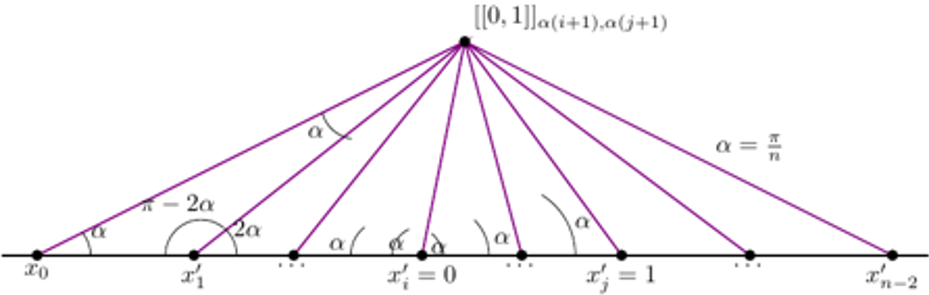
\includegraphics[
        width=0.8cm,
        height=0.8cm
    ]{structure/method_figures/predicted_rl_8_new.png}%
};

\node[
    img,
    anchor=north
] (rlpredtwo)
at ($(rlpredone.south)+(0,-0.1cm)$)
{%
    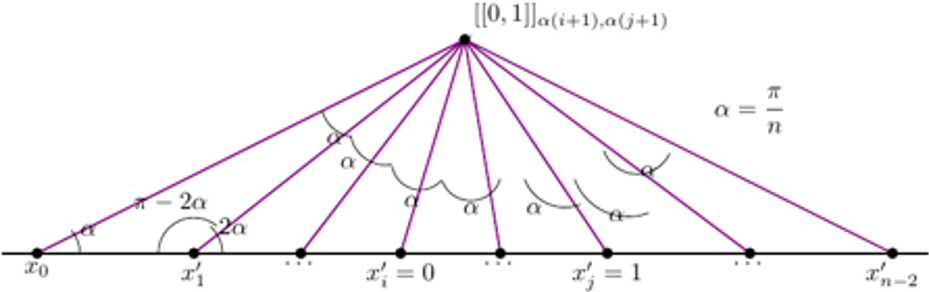
\includegraphics[
        width=0.8cm,
        height=0.8cm
    ]{structure/method_figures/predicted_rl_2_new.png}%
};

\node[
    img,
    anchor=north
] (rlpredthree)
at ($(rlpredtwo.south)+(0,-0.1cm)$)
{%
    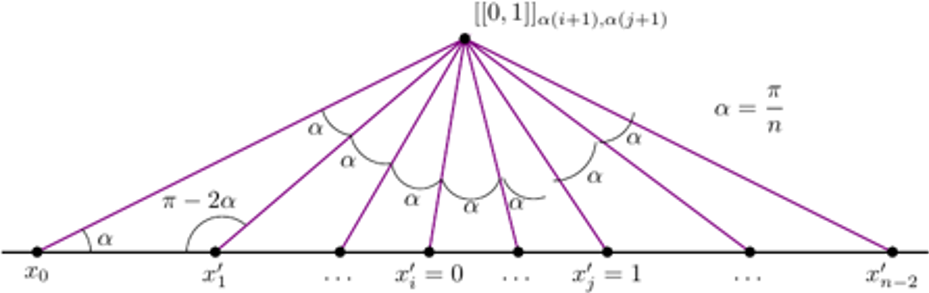
\includegraphics[
        width=0.8cm,
        height=0.8cm
    ]{structure/method_figures/predicted_rl_6_new.png}%
};

\node[
    img,
    anchor=north
] (rlpredfour)
at ($(rlpredthree.south)+(0,-0.10cm)$)
{%
    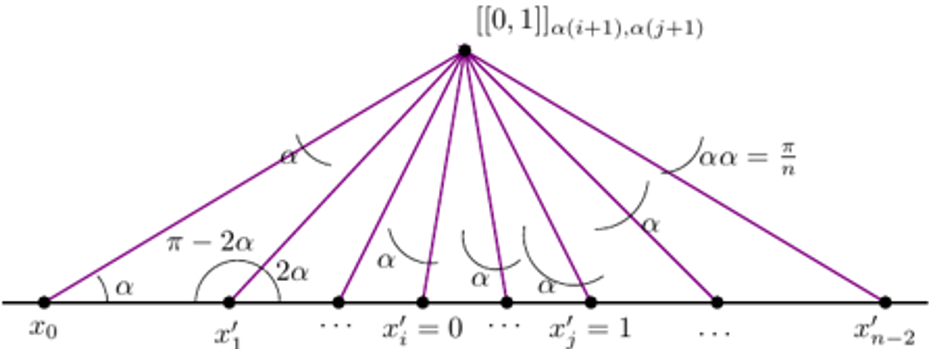
\includegraphics[
        width=0.8cm,
        height=0.8cm
    ]{structure/method_figures/predicted_rl_4_new.png}%
};

\node[
    anchor=north,
    font=\small
] at ($(rlpredfour.south)+(0.0,0.12cm)$)
{\shortstack{$\cdot$\\[-5pt]$\cdot$\\[-5pt]$\cdot$}};

\draw[forward]
    ($(compiler.east)+(0.0,-0.4cm)$)
    -- 
    (rolloutbox.west);

\node[
    frozenie,
    anchor=west
] (IEbottom)
at ($(rolloutbox.east)+(0.20cm,0)$)
{IE};

\draw[forward]
    (rolloutbox.east)
    --
    (IEbottom.west);

\node[
    circle,
    fill=black,
    inner sep=0.7pt
] (RLPortalLower)
at ($(IEbottom.south)+(0,-0.16cm)$) {};

\draw[
    connector,
    densely dotted
]
(IEbottom.south) -- (RLPortalLower.north);

\node[
    frozenie,
    anchor=west
] (IEtop)
at ($(IEbottom.west)+(0,1.3cm)$)
{IE};

\node[
    rolloutbox,
    anchor=east,
    minimum width=0.85cm,
    minimum height=0.42cm
] (targetbox)
at ($(IEtop.west)+(-0.20cm,0)$) {};

\node[
    branchtitle,
    anchor=south
]
at ($(targetbox.north)+(0,0.03cm)$)
{Ground Truth};

\node[
    img,
    anchor=center
] (rltarget)
at (targetbox.center)
{%
    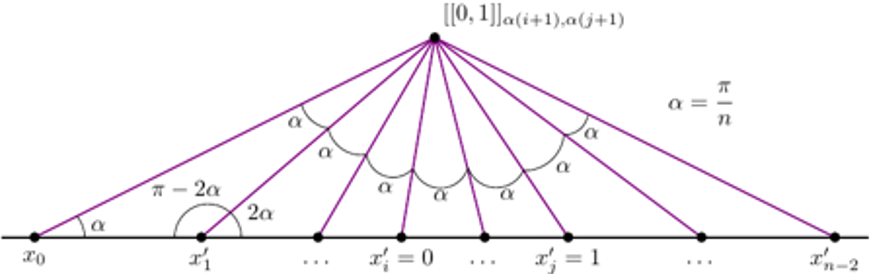
\includegraphics[
        width=0.8cm,
        height=0.8cm
    ]{structure/method_figures/target_rl_new.png}%
};

\draw[forward]
    (targetbox.east)
    --
    (IEtop.west);

\node[
    circle,
    fill=black,
    inner sep=0.7pt
] (RLPortalUpper)
at ($(IEtop.south)+(0,-0.16cm)$) {};

\draw[
    connector,
    densely dotted
]
(IEtop.south) -- (RLPortalUpper.north);

\node[
    font=\bfseries\tiny
] (Rsim)
at ($(IEtop.east)!0.5!(IEbottom.east)+(0.7cm,0)$)
{\(\mathcal{R}_{\mathrm{SSim}}\)};

\draw[forward]
    (IEtop.east)
    to[out=10,in=150]
    ($(Rsim.west)+(0.1cm,0)$);

\draw[forward]
    (IEbottom.east)
    to[out=-10,in=210]
    ($(Rsim.west)+(0.1cm,0)$);

\node[
    judgevlm,
    anchor=west
] (VLMJudge)
at ($(IEbottom.south)+(1.4,-0.3cm)$) {Judge};

\draw[forward]
    ($(rolloutbox.east)+(0.0,-0.65cm)$)
    -- 
    ($(VLMJudge.west)+(0.0,-0.15cm)$);

\node[
    star,
    fill=black,
    inner sep=0.7pt
] (JudgePortalTwo)
at ($(VLMJudge.west)+(-0.2,0.15cm)$) {};

\draw[
    connector,
    densely dotted
]
(JudgePortalTwo.east) -- ($(VLMJudge.west)+(0.0,0.15cm)$);

\node[
    prompt,
    anchor=north,
    text width=1.45cm,
    minimum height=0.85cm,
    font=\fontsize{3}{3.5}\selectfont
] (judgeprompt)
at ($(VLMJudge.north)+(0.3,1.8cm)$)
{You are a strict visual reward judge for scientific figure editing. \\
You are given two images: \\
- Image 1 is the source figure before editing. \\
- Image 2 is the predicted figure after editing. \\
You are also given a list of requested atomic edits. \\
Judge whether Image 2 applies each requested atomic edit relative to Image 1...};

\draw[forward]
    ($(judgeprompt.south)+(-0.3cm,0)$)
    to
    (VLMJudge.north);

\node[
    font=\bfseries\tiny
] (Rjudge)
at ($(VLMJudge.east)+(0.59cm,0)$)
{\(\mathcal{R}_{\mathrm{AE}}\)};

\draw[forward]
    (VLMJudge.east)
    to
    ($(Rjudge.west)+(0.1cm,0)$);

\end{tikzpicture}
\end{adjustbox}

\caption{Two-stage training pipeline. Left: Multi-task SFT jointly trains on equal amounts of editing (DaEdiTikZ) and reconstruction (DaTikZ-V4) data. Right: GDPO optimizes on a disjoint DaEdiTikZ subset using SelfSim from the frozen SFT vision encoder and instruction-following from a VLM judge.}
\label{fig:method_figure}

\end{figure*}